\documentclass[../tex_main/NEMO_manual]{subfiles}
\begin{document}
% ================================================================
% Appendix E : Note on some algorithms
% ================================================================
\chapter{Note on some algorithms}
\label{apdx:E}
\minitoc

\newpage
$\ $\newline    % force a new ligne
 
 This appendix some on going consideration on algorithms used or planned to be used
in \NEMO. 

$\ $\newline    % force a new ligne

% -------------------------------------------------------------------------------------------------------------
%        UBS scheme  
% -------------------------------------------------------------------------------------------------------------
\section{Upstream Biased Scheme (UBS) (\protect\np{ln\_traadv\_ubs}\forcode{ = .true.})}
\label{sec:TRA_adv_ubs}

The UBS advection scheme is an upstream biased third order scheme based on 
an upstream-biased parabolic interpolation. It is also known as Cell Averaged 
QUICK scheme (Quadratic Upstream Interpolation for Convective 
Kinematics). For example, in the $i$-direction :
\begin{equation} \label{eq:tra_adv_ubs2}
\tau _u^{ubs} = \left\{	 \begin{aligned}
  & \tau _u^{cen4} + \frac{1}{12} \,\tau"_i	   & \quad \text{if }\ u_{i+1/2} \geqslant 0 \\
  & \tau _u^{cen4} - \frac{1}{12} \,\tau"_{i+1} & \quad \text{if }\ u_{i+1/2}       <       0
  						 \end{aligned}    \right.
\end{equation}
or equivalently, the advective flux is
\begin{equation} \label{eq:tra_adv_ubs2}
U_{i+1/2} \ \tau _u^{ubs} 
=U_{i+1/2} \ \overline{ T_i - \frac{1}{6}\,\tau"_i }^{\,i+1/2}
- \frac{1}{2}\, |U|_{i+1/2} \;\frac{1}{6} \;\delta_{i+1/2}[\tau"_i]
\end{equation}
where $U_{i+1/2} = e_{1u}\,e_{3u}\,u_{i+1/2}$ and 
$\tau "_i =\delta _i \left[ {\delta _{i+1/2} \left[ \tau \right]} \right]$. 
By choosing this expression for $\tau "$ we consider a fourth order approximation 
of $\partial_i^2$ with a constant i-grid spacing ($\Delta i=1$). 

Alternative choice: introduce the scale factors:  
$\tau "_i =\frac{e_{1T}}{e_{2T}\,e_{3T}}\delta _i \left[ \frac{e_{2u} e_{3u} }{e_{1u} }\delta _{i+1/2}[\tau] \right]$.


This results in a dissipatively dominant (i.e. hyper-diffusive) truncation 
error \citep{Shchepetkin_McWilliams_OM05}. The overall performance of the 
advection scheme is similar to that reported in \cite{Farrow1995}. 
It is a relatively good compromise between accuracy and smoothness. It is 
not a \emph{positive} scheme meaning false extrema are permitted but the 
amplitude of such are significantly reduced over the centred second order 
method. Nevertheless it is not recommended to apply it to a passive tracer 
that requires positivity. 

The intrinsic diffusion of UBS makes its use risky in the vertical direction 
where the control of artificial diapycnal fluxes is of paramount importance. 
It has therefore been preferred to evaluate the vertical flux using the TVD 
scheme when \np{ln\_traadv\_ubs}\forcode{ = .true.}.

For stability reasons, in \autoref{eq:tra_adv_ubs}, the first term which corresponds 
to a second order centred scheme is evaluated using the \textit{now} velocity 
(centred in time) while the second term which is the diffusive part of the scheme, 
is evaluated using the \textit{before} velocity (forward in time. This is discussed 
by \citet{Webb_al_JAOT98} in the context of the Quick advection scheme. UBS and QUICK 
schemes only differ by one coefficient. Substituting 1/6 with 1/8 in 
(\autoref{eq:tra_adv_ubs}) leads to the QUICK advection scheme \citep{Webb_al_JAOT98}. 
This option is not available through a namelist parameter, since the 1/6 
coefficient is hard coded. Nevertheless it is quite easy to make the 
substitution in \mdl{traadv\_ubs} module and obtain a QUICK scheme

NB 1: When a high vertical resolution $O(1m)$ is used, the model stability can 
be controlled by vertical advection (not vertical diffusion which is usually 
solved using an implicit scheme). Computer time can be saved by using a 
time-splitting technique on vertical advection. This possibility have been 
implemented and validated in ORCA05-L301. It is not currently offered in the 
current reference version. 

NB 2 : In a forthcoming release four options will be proposed for the 
vertical component used in the UBS scheme. $\tau _w^{ubs}$ will be 
evaluated using either \textit{(a)} a centred $2^{nd}$ order scheme , 
or  \textit{(b)} a TVD scheme, or  \textit{(c)} an interpolation based on conservative 
parabolic splines following \citet{Shchepetkin_McWilliams_OM05} implementation of UBS in ROMS, 
or  \textit{(d)} an UBS. The $3^{rd}$ case has dispersion properties similar to an 
eight-order accurate conventional scheme.

NB 3 : It is straight forward to rewrite \autoref{eq:tra_adv_ubs} as follows:
\begin{equation} \label{eq:tra_adv_ubs2}
\tau _u^{ubs} = \left\{	 \begin{aligned}
	& \tau _u^{cen4} + \frac{1}{12} \tau"_i		& \quad \text{if }\ u_{i+1/2} \geqslant 0 \\
	& \tau _u^{cen4} - \frac{1}{12} \tau"_{i+1}	& \quad \text{if }\ u_{i+1/2}       <       0
  						 \end{aligned}    \right.
\end{equation}
or equivalently 
\begin{equation} \label{eq:tra_adv_ubs2}
\begin{split}
e_{2u} e_{3u}\,u_{i+1/2} \ \tau _u^{ubs} 
&= e_{2u} e_{3u}\,u_{i+1/2} \ \overline{ T - \frac{1}{6}\,\tau"_i }^{\,i+1/2} \\
& - \frac{1}{2} e_{2u} e_{3u}\,|u|_{i+1/2} \;\frac{1}{6} \;\delta_{i+1/2}[\tau"_i]
\end{split}
\end{equation}
\autoref{eq:tra_adv_ubs2} has several advantages. First it clearly evidence that 
the UBS scheme is based on the fourth order scheme to which is added an 
upstream biased diffusive term. Second, this emphasises that the $4^{th}$ order 
part have to be evaluated at \emph{now} time step, not only the $2^{th}$ order 
part as stated above using \autoref{eq:tra_adv_ubs}. Third, the diffusive term is 
in fact a biharmonic operator with a eddy coefficient with is simply proportional 
to the velocity.

laplacian diffusion:
\begin{equation} \label{eq:tra_ldf_lap}
\begin{split}
D_T^{lT} =\frac{1}{e_{1T} \; e_{2T}\;  e_{3T} } &\left[ {\quad \delta _i 
\left[ {A_u^{lT} \frac{e_{2u} e_{3u} }{e_{1u} }\;\delta _{i+1/2} 
\left[ T \right]} \right]} \right.
\\
&\ \left. {+\; \delta _j \left[ 
{A_v^{lT} \left( {\frac{e_{1v} e_{3v} }{e_{2v} }\;\delta _{j+1/2} \left[ T 
\right]} \right)} \right]\quad } \right]
\end{split}
\end{equation}

bilaplacian:
\begin{equation} \label{eq:tra_ldf_lap}
\begin{split}
D_T^{lT} =&-\frac{1}{e_{1T} \; e_{2T}\;  e_{3T}} \\
& \delta _i \left[  \sqrt{A_u^{lT}}\ \frac{e_{2u}\,e_{3u}}{e_{1u}}\;\delta _{i+1/2} 
		  \left[ \frac{1}{e_{1T}\,e_{2T}\, e_{3T}}
    \delta _i \left[ \sqrt{A_u^{lT}}\ \frac{e_{2u}\,e_{3u}}{e_{1u}}\;\delta _{i+1/2} 
    		  [T] \right] \right] \right]
\end{split}
\end{equation}
with ${A_u^{lT}}^2 = \frac{1}{12} {e_{1u}}^3\ |u|$, 
$i.e.$ $A_u^{lT} = \frac{1}{\sqrt{12}} \,e_{1u}\ \sqrt{ e_{1u}\,|u|\,}$
it comes :
\begin{equation} \label{eq:tra_ldf_lap}
\begin{split}
D_T^{lT} =&-\frac{1}{12}\,\frac{1}{e_{1T} \; e_{2T}\;  e_{3T}} \\
& \delta _i \left[ e_{2u}\,e_{3u}\,\sqrt{ e_{1u}\,|u|\,}\;\delta _{i+1/2} 
		 \left[ \frac{1}{e_{1T}\,e_{2T}\, e_{3T}} 
    \delta _i \left[ e_{2u}\,e_{3u}\,\sqrt{ e_{1u}\,|u|\,}\;\delta _{i+1/2} 
    		[T] \right] \right] \right]
\end{split}
\end{equation}
if the velocity is uniform ($i.e.$ $|u|=cst$) then the diffusive flux is
\begin{equation} \label{eq:tra_ldf_lap}
\begin{split}
F_u^{lT} = - \frac{1}{12}
 e_{2u}\,e_{3u}\,|u| \;\sqrt{ e_{1u}}\,\delta _{i+1/2} 
		 \left[ \frac{1}{e_{1T}\,e_{2T}\, e_{3T}} 
    \delta _i \left[ e_{2u}\,e_{3u}\,\sqrt{ e_{1u}}\:\delta _{i+1/2} 
    		[T] \right] \right]
\end{split}
\end{equation}
beurk....  reverte the logic: starting from the diffusive part of the advective flux it comes:

\begin{equation} \label{eq:tra_adv_ubs2}
\begin{split}
F_u^{lT}
&= - \frac{1}{2} e_{2u} e_{3u}\,|u|_{i+1/2} \;\frac{1}{6} \;\delta_{i+1/2}[\tau"_i]
\end{split}
\end{equation}
if the velocity is uniform ($i.e.$ $|u|=cst$) and choosing $\tau "_i =\frac{e_{1T}}{e_{2T}\,e_{3T}}\delta _i \left[ \frac{e_{2u} e_{3u} }{e_{1u} } \delta _{i+1/2}[\tau] \right]$

sol 1 coefficient at T-point ( add $e_{1u}$ and $e_{1T}$ on both side of first $\delta$):
\begin{equation} \label{eq:tra_adv_ubs2}
\begin{split}
F_u^{lT}
&= - \frac{1}{12} \frac{e_{2u} e_{3u}}{e_{1u}}\;\delta_{i+1/2}\left[ \frac{e_{1T}^3\,|u|}{e_{1T}e_{2T}\,e_{3T}}\,\delta _i \left[ \frac{e_{2u} e_{3u} }{e_{1u} } \delta _{i+1/2}[\tau] \right] \right]
\end{split}
\end{equation}
which leads to ${A_T^{lT}}^2 = \frac{1}{12} {e_{1T}}^3\ \overline{|u|}^{\,i+1/2}$

sol 2 coefficient at u-point: split $|u|$ into $\sqrt{|u|}$ and $e_{1T}$ into $\sqrt{e_{1u}}$
\begin{equation} \label{eq:tra_adv_ubs2}
\begin{split}
F_u^{lT}
&= - \frac{1}{12} {e_{1u}}^1 \sqrt{e_{1u}|u|} \frac{e_{2u} e_{3u}}{e_{1u}}\;\delta_{i+1/2}\left[ \frac{1}{e_{2T}\,e_{3T}}\,\delta _i \left[ \sqrt{e_{1u}|u|} \frac{e_{2u} e_{3u} }{e_{1u} } \delta _{i+1/2}[\tau] \right] \right] \\
&= - \frac{1}{12} e_{1u} \sqrt{e_{1u}|u|\,} \frac{e_{2u} e_{3u}}{e_{1u}}\;\delta_{i+1/2}\left[ \frac{1}{e_{1T}\,e_{2T}\,e_{3T}}\,\delta _i \left[ e_{1u} \sqrt{e_{1u}|u|\,} \frac{e_{2u} e_{3u} }{e_{1u}} \delta _{i+1/2}[\tau] \right] \right]
\end{split}
\end{equation}
which leads to ${A_u^{lT}} = \frac{1}{12} {e_{1u}}^3\ |u|$


% -------------------------------------------------------------------------------------------------------------
%        Leap-Frog energetic  
% -------------------------------------------------------------------------------------------------------------
\section{Leapfrog energetic}
\label{sec:LF}

We adopt the following semi-discrete notation for time derivative. Given the values of a variable $q$ at successive time step, the time derivation and averaging operators at the mid time step are:
\begin{subequations} \label{eq:dt_mt}
\begin{align}
 \delta _{t+\rdt/2} [q]     &=  \  \ \,   q^{t+\rdt}  - q^{t}		\\
 \overline q^{\,t+\rdt/2} &= \left\{ q^{t+\rdt} + q^{t} \right\} \; / \; 2
\end{align}
\end{subequations}
As for space operator, the adjoint of the derivation and averaging time operators are 
$\delta_t^*=\delta_{t+\rdt/2}$ and $\overline{\cdot}^{\,t\,*}= \overline{\cdot}^{\,t+\Delta/2}$
, respectively. 

The Leap-frog time stepping given by \autoref{eq:DOM_nxt} can be defined as:
\begin{equation} \label{eq:LF}
   \frac{\partial q}{\partial t} 
   		\equiv \frac{1}{\rdt} \overline{ \delta _{t+\rdt/2}[q]}^{\,t} 
		=         \frac{q^{t+\rdt}-q^{t-\rdt}}{2\rdt}
\end{equation} 
Note that \autoref{chap:LF} shows that the leapfrog time step is $\rdt$, not $2\rdt$ 
as it can be found sometime in literature. 
The leap-Frog time stepping is a second order centered scheme. As such it respects 
the quadratic invariant in integral forms, $i.e.$ the following continuous property,
\begin{equation} \label{eq:Energy}
\int_{t_0}^{t_1} {q\, \frac{\partial q}{\partial t} \;dt} 
	=\int_{t_0}^{t_1} {\frac{1}{2}\, \frac{\partial q^2}{\partial t} \;dt} 
	=  \frac{1}{2} \left( {q_{t_1}}^2 - {q_{t_0}}^2 \right) ,
\end{equation}
is satisfied in discrete form. Indeed, 
\begin{equation} \begin{split}
\int_{t_0}^{t_1} {q\, \frac{\partial q}{\partial t} \;dt} 
	&\equiv \sum\limits_{0}^{N} 
			{\frac{1}{\rdt} q^t \ \overline{ \delta _{t+\rdt/2}[q]}^{\,t} \ \rdt} 
	   \equiv \sum\limits_{0}^{N}  { q^t \ \overline{ \delta _{t+\rdt/2}[q]}^{\,t} } \\
	&\equiv \sum\limits_{0}^{N}  { \overline{q}^{\,t+\Delta/2}{ \delta _{t+\rdt/2}[q]}}
	   \equiv \sum\limits_{0}^{N}  { \frac{1}{2} \delta _{t+\rdt/2}[q^2] }\\
	&\equiv \sum\limits_{0}^{N}  { \frac{1}{2} \delta _{t+\rdt/2}[q^2] }
	   \equiv \frac{1}{2} \left( {q_{t_1}}^2 - {q_{t_0}}^2 \right)
\end{split} \end{equation}
NB here pb of boundary condition when applying the adjoin! In space, setting to 0 
the quantity in land area is sufficient to get rid of the boundary condition 
(equivalently of the boundary value of the integration by part). In time this boundary 
condition is not physical and \textbf{add something here!!!}






% ================================================================
% Iso-neutral diffusion : 
% ================================================================

\section{Lateral diffusion operator}

% ================================================================
% Griffies' iso-neutral diffusion operator : 
% ================================================================
\subsection{Griffies iso-neutral diffusion operator}

Let try to define a scheme that get its inspiration from the \citet{Griffies_al_JPO98}
scheme, but is formulated within the \NEMO framework ($i.e.$ using scale 
factors rather than grid-size and having a position of $T$-points that is not 
necessary in the middle of vertical velocity points, see \autoref{fig:zgr_e3}).

In the formulation \autoref{eq:tra_ldf_iso} introduced in 1995 in OPA, the ancestor of \NEMO, 
the off-diagonal terms of the small angle diffusion tensor contain several double 
spatial averages of a gradient, for example $\overline{\overline{\delta_k \cdot}}^{\,i,k}$. 
It is apparent that the combination of a $k$ average and a $k$ derivative of the tracer 
allows for the presence of grid point oscillation structures that will be invisible 
to the operator. These structures are \textit{computational modes}. They
will not be damped by the iso-neutral operator, and even possibly amplified by it. 
In other word, the operator applied to a tracer does not warranties the decrease of 
its global average variance. To circumvent this, we have introduced a smoothing of 
the slopes of the iso-neutral surfaces (see \autoref{chap:LDF}). Nevertheless, this technique 
works fine for $T$ and $S$ as they are active tracers ($i.e.$ they enter the computation 
of density), but it does not work for a passive tracer.   \citep{Griffies_al_JPO98} introduce 
a different way to discretise the off-diagonal terms that nicely solve the problem. 
The idea is to get rid of combinations of an averaged in one direction combined 
with a derivative in the same direction by considering triads. For example in the 
(\textbf{i},\textbf{k}) plane, the four triads are defined at the $(i,k)$ $T$-point as follows:
\begin{equation} \label{eq:Gf_triads}
_i^k \mathbb{T}_{i_p}^{k_p} (T)
= \frac{1}{4} \ {b_u}_{\,i+i_p}^{\,k}  \  A_i^k  	\left(  
                                                     \frac{ \delta_{i + i_p}[T^k] }{ {e_{1u}}_{\,i + i_p}^{\,k} } 
-\ {_i^k \mathbb{R}_{i_p}^{k_p}} \ \frac{ \delta_{k+k_p} [T^i] }{ {e_{3w}}_{\,i}^{\,k+k_p} } 
									  \right)
\end{equation}
where the indices $i_p$ and $k_p$ define the four triads and take the following value: 
$i_p = -1/2$ or $1/2$ and $k_p = -1/2$ or $1/2$, 
$b_u= e_{1u}\,e_{2u}\,e_{3u}$ is the volume of $u$-cells, 
$A_i^k$ is the lateral eddy diffusivity coefficient defined at $T$-point,
and $_i^k \mathbb{R}_{i_p}^{k_p}$ is the slope associated with each triad :
\begin{equation} \label{eq:Gf_slopes}
_i^k \mathbb{R}_{i_p}^{k_p} 
=\frac{ {e_{3w}}_{\,i}^{\,k+k_p}} { {e_{1u}}_{\,i+i_p}^{\,k}} \ \frac 
{\left(\alpha / \beta \right)_i^k  \ \delta_{i + i_p}[T^k] - \delta_{i + i_p}[S^k] }
{\left(\alpha / \beta \right)_i^k  \ \delta_{k+k_p}[T^i ] - \delta_{k+k_p}[S^i ] }
\end{equation}
Note that in \autoref{eq:Gf_slopes} we use the ratio $\alpha / \beta$ instead of 
multiplying the temperature derivative by $\alpha$ and the salinity derivative 
by $\beta$. This is more efficient as the ratio $\alpha / \beta$ can to be 
evaluated directly.

Note that in \autoref{eq:Gf_triads}, we chose to use ${b_u}_{\,i+i_p}^{\,k}$ instead of 
${b_{uw}}_{\,i+i_p}^{\,k+k_p}$. This choice has been motivated by the decrease 
of tracer variance and the presence of partial cell at the ocean bottom 
(see \autoref{apdx:Gf_operator}).

%>>>>>>>>>>>>>>>>>>>>>>>>>>>>>>>>
\begin{figure}[!ht] \begin{center}
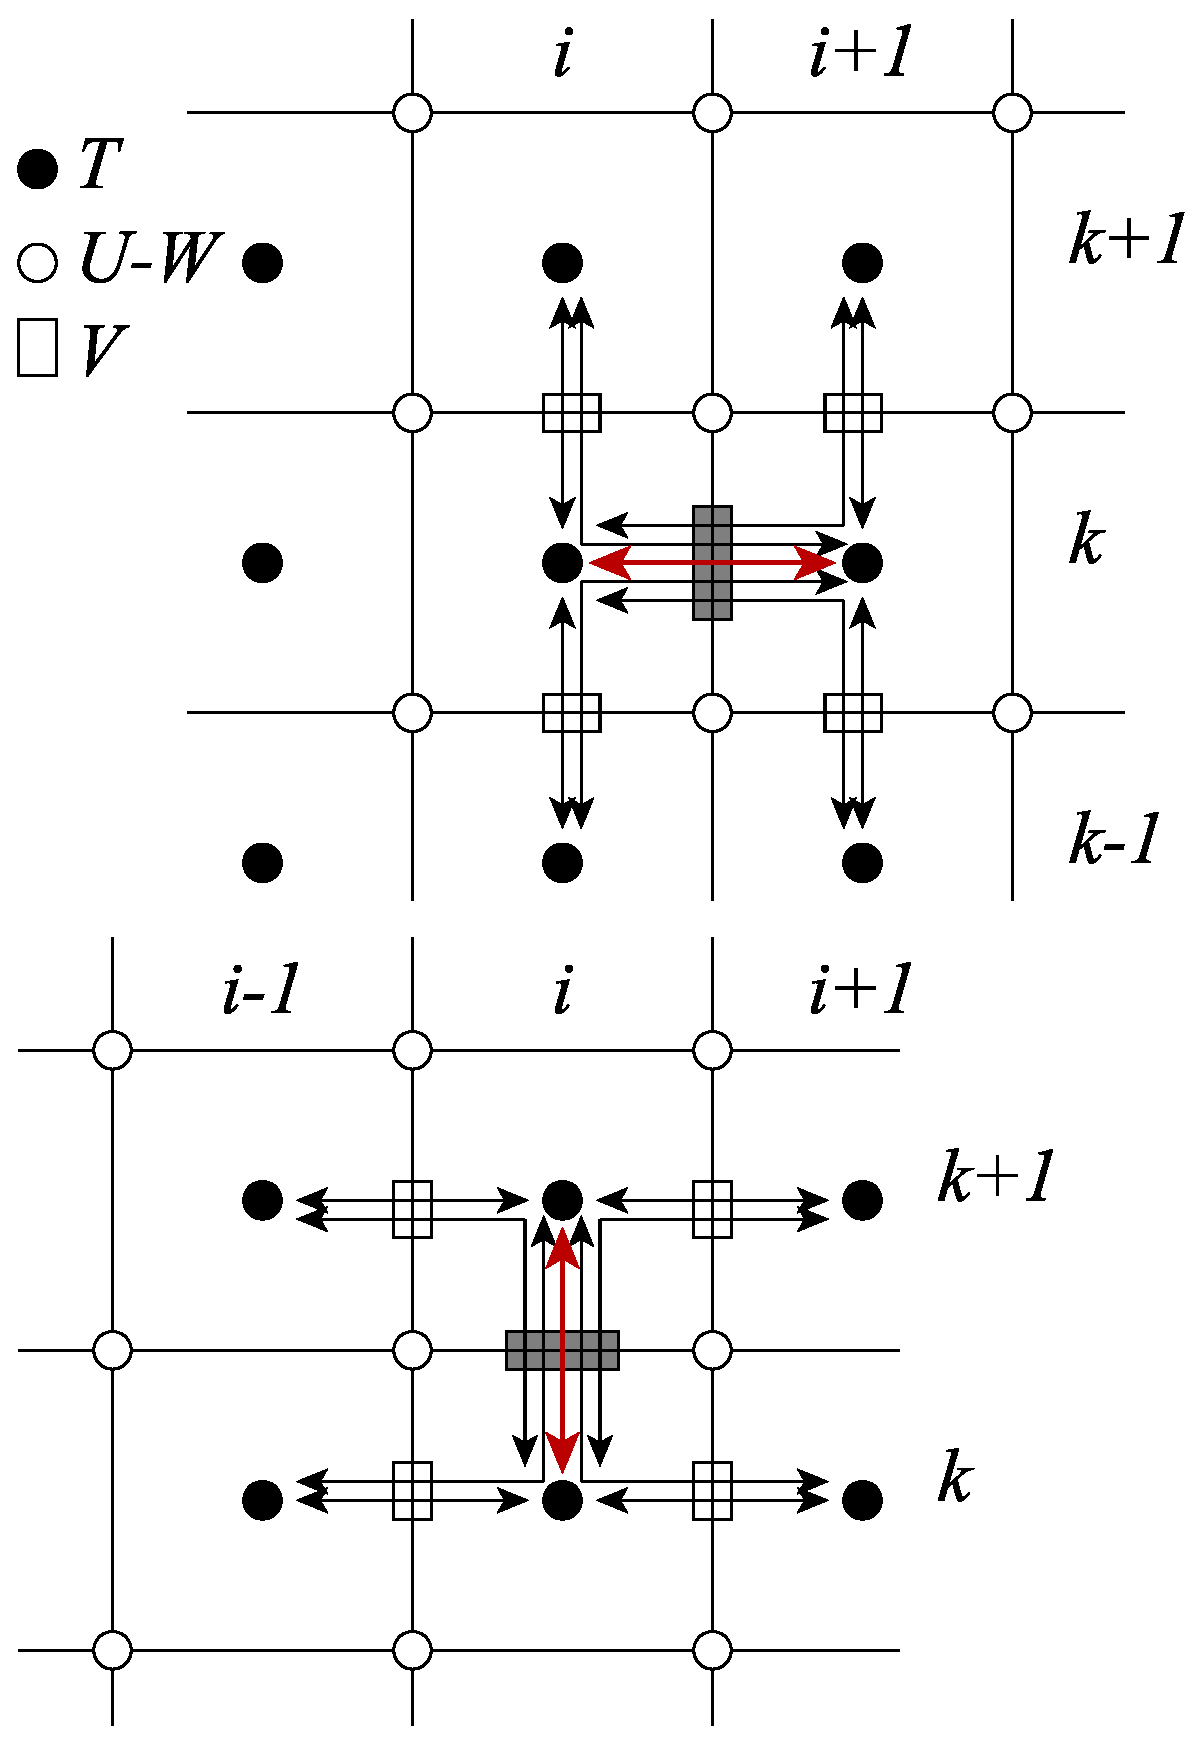
\includegraphics[width=0.70\textwidth]{Fig_ISO_triad}
\caption{  \protect\label{fig:ISO_triad}   
Triads used in the Griffies's like iso-neutral diffision scheme for 
$u$-component (upper panel) and $w$-component (lower panel).}
\end{center}
\end{figure}
%>>>>>>>>>>>>>>>>>>>>>>>>>>>>>>>>

The four iso-neutral fluxes associated with the triads are defined at $T$-point. 
They take the following expression :
\begin{flalign} \label{eq:Gf_fluxes}
\begin{split}
{_i^k {\mathbb{F}_u}_{i_p}^{k_p} } (T) 
   &= \ \; \qquad  \quad    { _i^k \mathbb{T}_{i_p}^{k_p} }(T) \;\ / \ { {e_{1u}}_{\,i+i_p}^{\,k}}    \\
{_i^k {\mathbb{F}_w}_{i_p}^{k_p} } (T)
   &=  -\; { _i^k \mathbb{R}_{i_p}^{k_p} }
				 \ \; { _i^k \mathbb{T}_{i_p}^{k_p} }(T) \;\ / \ { {e_{3w}}_{\,i}^{\,k+k_p}}
\end{split}
\end{flalign}

The resulting iso-neutral fluxes at $u$- and $w$-points are then given by the 
sum of the fluxes that cross the $u$- and $w$-face (\autoref{fig:ISO_triad}):
\begin{flalign} \label{eq:iso_flux} 
\textbf{F}_{iso}(T) 
&\equiv  \sum_{\substack{i_p,\,k_p}} 
   \begin{pmatrix} 
      {_{i+1/2-i_p}^k {\mathbb{F}_u}_{i_p}^{k_p} } (T)      \\
      \\
      {_i^{k+1/2-k_p} {\mathbb{F}_w}_{i_p}^{k_p} } (T)      \\   
   \end{pmatrix}    \notag \\
&  \notag \\
&\equiv  \sum_{\substack{i_p,\,k_p}} 
   \begin{pmatrix} 
      && { _{i+1/2-i_p}^k \mathbb{T}_{i_p}^{k_p} }(T) \;\ / \ { {e_{1u}}_{\,i+1/2}^{\,k} }    \\
      \\
      & -\; { _i^{k+1/2-k_p} \mathbb{R}_{i_p}^{k_p} }
        & {_i^{k+1/2-k_p} \mathbb{T}_{i_p}^{k_p} }(T) \;\ / \ { {e_{3w}}_{\,i}^{\,k+1/2} }   \\   
   \end{pmatrix}      % \\
% &\\
% &\equiv  \sum_{\substack{i_p,\,k_p}} 
%    \begin{pmatrix} 
%       \qquad  \qquad  \qquad 
%       \frac{1}{ {e_{1u}}_{\,i+1/2}^{\,k} }  \ \;  
%        { _{i+1/2-i_p}^k \mathbb{T}_{i_p}^{k_p} }(T)\\
%       \\
%       -\frac{1}{ {e_{3w}}_{\,i}^{\,k+1/2} }  \ \; 
%        { _i^{k+1/2-k_p} \mathbb{R}_{i_p}^{k_p} } \ \;  
%                  {_i^{k+1/2-k_p} \mathbb{T}_{i_p}^{k_p} }(T)\\   
%    \end{pmatrix}      
\end{flalign}
resulting in a iso-neutral diffusion tendency on temperature given by the divergence 
of the sum of all the four triad fluxes :
\begin{equation} \label{eq:Gf_operator}
D_l^T = \frac{1}{b_T}  \sum_{\substack{i_p,\,k_p}} \left\{  
		 \delta_{i} \left[{_{i+1/2-i_p}^k {\mathbb{F}_u }_{i_p}^{k_p}} \right] 
	     + \delta_{k} \left[ {_i^{k+1/2-k_p} {\mathbb{F}_w}_{i_p}^{k_p}} \right]   \right\}
\end{equation}
where $b_T= e_{1T}\,e_{2T}\,e_{3T}$ is the volume of $T$-cells. 

This expression of the iso-neutral diffusion has been chosen in order to satisfy 
the following six properties:
\begin{description}
\item[$\bullet$ horizontal diffusion] The discretization of the diffusion operator 
recovers the traditional five-point Laplacian in the limit of flat iso-neutral direction :
\begin{equation} \label{eq:Gf_property1a}
D_l^T = \frac{1}{b_T}  \ \delta_{i} 
	\left[ \frac{e_{2u}\,e_{3u}}{e_{1u}} \; \overline{A}^{\,i} \; \delta_{i+1/2}[T] \right] 
\qquad  \text{when} \quad 
	{ _i^k \mathbb{R}_{i_p}^{k_p} }=0
\end{equation}

\item[$\bullet$ implicit treatment in the vertical]  In the diagonal term associated 
with the vertical divergence of the iso-neutral fluxes (i.e. the term associated 
with a second order vertical derivative) appears only tracer values associated 
with a single water column. This is of paramount importance since it means
that the implicit in time algorithm for solving the vertical diffusion equation can 
be used to evaluate this term. It is a necessity since the vertical eddy diffusivity 
associated with this term,  
\begin{equation}
	 \sum_{\substack{i_p, \,k_p}} \left\{  
		A_i^k \; \left(_i^k \mathbb{R}_{i_p}^{k_p}\right)^2
	\right\} 
\end{equation}
can be quite large.

\item[$\bullet$ pure iso-neutral operator]  The iso-neutral flux of locally referenced 
potential density is zero, $i.e.$
\begin{align} \label{eq:Gf_property2}
\begin{matrix}
&{_i^k {\mathbb{F}_u}_{i_p}^{k_p} (\rho)} 
	&=    &\alpha_i^k   &{_i^k {\mathbb{F}_u}_{i_p}^{k_p} } (T) 
	&- \ \;  \beta _i^k    &{_i^k {\mathbb{F}_u}_{i_p}^{k_p} } (S) & = \ 0   \\
&{_i^k {\mathbb{F}_w}_{i_p}^{k_p} (\rho)} 
	&=    &\alpha_i^k   &{_i^k {\mathbb{F}_w}_{i_p}^{k_p} } (T) 
	&- \  \; \beta _i^k    &{_i^k {\mathbb{F}_w}_{i_p}^{k_p} } (S)  &= \ 0
\end{matrix}
\end{align}
This result is trivially obtained using the \autoref{eq:Gf_triads} applied to $T$ and $S$ 
and the definition of the triads' slopes \autoref{eq:Gf_slopes}.

\item[$\bullet$ conservation of tracer] The iso-neutral diffusion term conserve the 
total tracer content, $i.e.$
\begin{equation} \label{eq:Gf_property1}
\sum_{i,j,k} \left\{ D_l^T \ b_T \right\} = 0
\end{equation}
This property is trivially satisfied since the iso-neutral diffusive operator 
is written in flux form.

\item[$\bullet$ decrease of tracer variance] The iso-neutral diffusion term does 
not increase the total tracer variance, $i.e.$
\begin{equation} \label{eq:Gf_property1}
\sum_{i,j,k} \left\{ T \ D_l^T \ b_T \right\} \leq 0
\end{equation}
The property is demonstrated in the \autoref{apdx:Gf_operator}. It is a 
key property for a diffusion term. It means that the operator is also a dissipation 
term, $i.e.$ it is a sink term for the square of the quantity on which it is applied. 
It therfore ensure that, when the diffusivity coefficient is large enough, the field 
on which it is applied become free of grid-point noise.

\item[$\bullet$ self-adjoint operator] The iso-neutral diffusion operator is self-adjoint, 
$i.e.$
\begin{equation} \label{eq:Gf_property1}
\sum_{i,j,k} \left\{ S \ D_l^T \ b_T \right\} = \sum_{i,j,k} \left\{ D_l^S \ T \ b_T \right\} 
\end{equation}
In other word, there is no needs to develop a specific routine from the adjoint of this 
operator. We just have to apply the same routine. This properties can be demonstrated 
quite easily in a similar way the "non increase of tracer variance" property has been 
proved (see \autoref{apdx:Gf_operator}).
\end{description}


$\ $\newline      %force an empty line
% ================================================================
% Skew flux formulation for Eddy Induced Velocity : 
% ================================================================
\subsection{Eddy induced velocity and skew flux formulation}

When Gent and McWilliams [1990] diffusion is used (\key{traldf\_eiv} defined), 
an additional advection term is added. The associated velocity is the so called 
eddy induced velocity, the formulation of which depends on the slopes of iso-
neutral surfaces. Contrary to the case of iso-neutral mixing, the slopes used 
here are referenced to the geopotential surfaces, $i.e.$ \autoref{eq:ldfslp_geo} 
is used in $z$-coordinate, and the sum \autoref{eq:ldfslp_geo}
+ \autoref{eq:ldfslp_iso} in $z^*$ or $s$-coordinates. 

The eddy induced velocity is given by: 
\begin{equation} \label{eq:eiv_v}
\begin{split}
 u^* & = - \frac{1}{e_2\,e_{3}}          \;\partial_k \left( e_2 \, A_e \; r_i  \right)   
          = - \frac{1}{e_3}                     \;\partial_k \left(           A_e \; r_i  \right)            \\
 v^* & = - \frac{1}{e_1\,e_3}\;             \partial_k \left( e_1 \, A_e \; r_j  \right)   
          = - \frac{1}{e_3}                     \;\partial_k \left(           A_e \; r_j  \right)             \\
w^* & =    \frac{1}{e_1\,e_2}\; \left\{   \partial_i  \left( e_2 \, A_e \; r_i  \right) 
					              + \partial_j  \left( e_1 \, A_e \;r_j   \right) \right\}   \\
\end{split}
\end{equation}
where $A_{e}$ is the eddy induced velocity coefficient, and $r_i$ and $r_j$ the 
slopes between the iso-neutral and the geopotential surfaces.
%%gm wrong: to be modified with 2 2D streamfunctions
 In other words,
the eddy induced velocity can be derived from a vector streamfuntion, $\phi$, which
is given by $\phi = A_e\,\textbf{r}$ as $\textbf{U}^*  = \textbf{k} \times \nabla \phi$
%%end gm

A traditional way to implement this additional advection is to add it to the eulerian 
velocity prior to compute the tracer advection. This allows us to take advantage of 
all the advection schemes offered for the tracers (see \autoref{sec:TRA_adv}) and not just 
a $2^{nd}$ order advection scheme. This is particularly useful for passive tracers 
where \emph{positivity} of the advection scheme is of paramount importance. 
% give here the expression using the triads. It is different from the one given in \autoref{eq:ldfeiv}
% see just below a copy of this equation:
%\begin{equation} \label{eq:ldfeiv}
%\begin{split}
% u^* & = \frac{1}{e_{2u}e_{3u}}\; \delta_k \left[e_{2u} \, A_{uw}^{eiv} \; \overline{r_{1w}}^{\,i+1/2} \right]\\
% v^* & = \frac{1}{e_{1u}e_{3v}}\; \delta_k \left[e_{1v} \, A_{vw}^{eiv} \; \overline{r_{2w}}^{\,j+1/2} \right]\\
%w^* & = \frac{1}{e_{1w}e_{2w}}\; \left\{ \delta_i \left[e_{2u} \, A_{uw}^{eiv} \; \overline{r_{1w}}^{\,i+1/2} \right] + %\delta_j \left[e_{1v} \, A_{vw}^{eiv} \; \overline{r_{2w}}^{\,j+1/2} \right] \right\} \\
%\end{split}
%\end{equation}
\begin{equation} \label{eq:eiv_vd}  
\textbf{F}_{eiv}^T   \equiv   \left( \begin{aligned}                                
 \sum_{\substack{i_p,\,k_p}} &
 +{e_{2u}}_{i+1/2-i_p}^{k}                                  \ \ {A_{e}}_{i+1/2-i_p}^{k} 
\ \ \ { _{i+1/2-i_p}^k \mathbb{R}_{i_p}^{k_p} }    \ \ \delta_{k+k_p}[T_{i+1/2-i_p}]      \\
    \\
 \sum_{\substack{i_p,\,k_p}} &
 - {e_{2u}}_i^{k+1/2-k_p}                                      \ {A_{e}}_i^{k+1/2-k_p} 
\ \ { _i^{k+1/2-k_p} \mathbb{R}_{i_p}^{k_p} }    \ \delta_{i+i_p}[T^{k+1/2-k_p}]    \\   
\end{aligned}   \right)
\end{equation}

\citep{Griffies_JPO98} introduces another way to implement the eddy induced advection, 
the so-called skew form. It is based on a transformation of the advective fluxes 
using the non-divergent nature of the eddy induced velocity. 
For example in the (\textbf{i},\textbf{k}) plane, the tracer advective fluxes can be 
transformed as follows:
\begin{flalign*}
\begin{split}
\textbf{F}_{eiv}^T = 
\begin{pmatrix} 
 	        {e_{2}\,e_{3}\;  u^*} 	 	\\
 		{e_{1}\,e_{2}\; w^*}	 \\
\end{pmatrix}   \;   T
&=
\begin{pmatrix} 
 	        { - \partial_k \left( e_{2} \, A_{e} \; r_i \right) \; T \;} 	 	\\
 		{+ \partial_i  \left( e_{2} \, A_{e} \; r_i \right) \; T \;}	 \\
\end{pmatrix} 			\\
&=			
\begin{pmatrix} 
 	        { - \partial_k \left( e_{2} \, A_{e} \; r_i  \; T \right) \;}  \\
 		{+ \partial_i  \left( e_{2} \, A_{e} \; r_i  \; T \right) \;}	 \\
\end{pmatrix} 			
 + 
\begin{pmatrix} 
 	        {+ e_{2} \, A_{e} \; r_i  \; \partial_k T}  \\
 		{ - e_{2} \, A_{e} \; r_i  \; \partial_i  T}	 \\
\end{pmatrix} 	 
\end{split}
\end{flalign*}
and since the eddy induces velocity field is no-divergent, we end up with the skew 
form of the eddy induced advective fluxes:
\begin{equation} \label{eq:eiv_skew_continuous}
\textbf{F}_{eiv}^T = \begin{pmatrix} 
 	        {+ e_{2} \, A_{e} \; r_i  \; \partial_k T}   \\
 		{ - e_{2} \, A_{e} \; r_i  \; \partial_i  T}	 \\
                                 \end{pmatrix}
\end{equation}
The tendency associated with eddy induced velocity is then simply the divergence 
of the \autoref{eq:eiv_skew_continuous} fluxes. It naturally conserves the tracer 
content, as it is expressed in flux form and, as the advective form, it preserve the 
tracer variance. Another interesting property of \autoref{eq:eiv_skew_continuous} 
form is that when $A=A_e$, a simplification occurs in the sum of the iso-neutral 
diffusion and eddy induced velocity terms:
\begin{flalign} \label{eq:eiv_skew+eiv_continuous}
\textbf{F}_{iso}^T + \textbf{F}_{eiv}^T &= 
\begin{pmatrix} 
 	        + \frac{e_2\,e_3\,}{e_1} A \;\partial_i T -  e_2 \, A \; r_i                              \;\partial_k T   \\
 		-  e_2 \, A_{e} \; r_i           \;\partial_i T + \frac{e_1\,e_2}{e_3} \, A \; r_i^2 \;\partial_k T   \\
\end{pmatrix}
+
\begin{pmatrix} 
 	        {+ e_{2} \, A_{e} \; r_i  \; \partial_k T}   \\
 		{ - e_{2} \, A_{e} \; r_i  \; \partial_i  T}	 \\
\end{pmatrix}      \\
&= \begin{pmatrix} 
 	        + \frac{e_2\,e_3\,}{e_1} A \;\partial_i T    \\
 		-  2\; e_2 \, A_{e} \; r_i      \;\partial_i T + \frac{e_1\,e_2}{e_3} \, A \; r_i^2 \;\partial_k T   \\
\end{pmatrix}
\end{flalign}
The horizontal component reduces to the one use for an horizontal laplacian 
operator and the vertical one keep the same complexity, but not more. This property
has been used to reduce the computational time \citep{Griffies_JPO98}, but it is 
not of practical use as usually $A \neq A_e$. Nevertheless this property can be used to 
choose a discret form of  \autoref{eq:eiv_skew_continuous} which is consistent with the 
iso-neutral operator \autoref{eq:Gf_operator}. Using the slopes \autoref{eq:Gf_slopes} 
and defining $A_e$ at $T$-point($i.e.$ as $A$, the eddy diffusivity coefficient),
the resulting discret form is given by:
\begin{equation} \label{eq:eiv_skew}  
\textbf{F}_{eiv}^T   \equiv   \frac{1}{4} \left( \begin{aligned}                                
 \sum_{\substack{i_p,\,k_p}} &
 +{e_{2u}}_{i+1/2-i_p}^{k}                                  \ \ {A_{e}}_{i+1/2-i_p}^{k} 
\ \ \ { _{i+1/2-i_p}^k \mathbb{R}_{i_p}^{k_p} }    \ \ \delta_{k+k_p}[T_{i+1/2-i_p}]      \\
    \\
 \sum_{\substack{i_p,\,k_p}} &
 - {e_{2u}}_i^{k+1/2-k_p}                                      \ {A_{e}}_i^{k+1/2-k_p} 
\ \ { _i^{k+1/2-k_p} \mathbb{R}_{i_p}^{k_p} }    \ \delta_{i+i_p}[T^{k+1/2-k_p}]    \\   
\end{aligned}   \right)
\end{equation}
Note that \autoref{eq:eiv_skew} is valid in $z$-coordinate with or without partial cells. 
In $z^*$ or $s$-coordinate, the slope between the level and the geopotential surfaces 
must be added to $\mathbb{R}$ for the discret form to be exact. 

Such a choice of discretisation is consistent with the iso-neutral operator as it uses the 
same definition for the slopes. It also ensures the conservation of the tracer variance 
(see Appendix \autoref{apdx:eiv_skew}), $i.e.$ it does not include a diffusive component 
but is a "pure" advection term.




$\ $\newpage      %force an empty line
% ================================================================
% Discrete Invariants of the iso-neutral diffrusion 
% ================================================================
\subsection{Discrete invariants of the iso-neutral diffrusion}
\label{subsec:Gf_operator}

Demonstration of the decrease of the tracer variance in the (\textbf{i},\textbf{j}) plane. 

This part will be moved in an Appendix.

The continuous property to be demonstrated is :
\begin{align*}
\int_D  D_l^T \; T \;dv   \leq 0
\end{align*}
The discrete form of its left hand side is obtained using \autoref{eq:iso_flux}

\begin{align*}
&\int_D  D_l^T \; T \;dv \equiv  \sum_{i,k} \left\{ T \ D_l^T \ b_T \right\}    \\
&\equiv + \sum_{i,k} \sum_{\substack{i_p,\,k_p}} \left\{  
		\delta_{i} \left[{_{i+1/2-i_p}^k {\mathbb{F}_u }_{i_p}^{k_p}} \right] 
	     + \delta_{k} \left[ {_i^{k+1/2-k_p} {\mathbb{F}_w}_{i_p}^{k_p}} \right]  \ T \right\}    \\
&\equiv  - \sum_{i,k} \sum_{\substack{i_p,\,k_p}} \left\{  
                {_{i+1/2-i_p}^k {\mathbb{F}_u }_{i_p}^{k_p}} \ \delta_{i+1/2} [T]
             + {_i^{k+1/2-k_p} {\mathbb{F}_w}_{i_p}^{k_p}}  \ \delta_{k+1/2} [T]   \right\}      \\
&\equiv -\sum_{i,k} \sum_{\substack{i_p,\,k_p}} \left\{  
	\frac{ _{i+1/2-i_p}^k \mathbb{T}_{i_p}^{k_p} (T) }{ {e_{1u}}_{\,i+1/2}^{\,k} }  \ \delta_{i+1/2} [T]
 - { _i^{k+1/2-k_p} \mathbb{R}_{i_p}^{k_p} } \ \; 
	\frac{ _i^{k+1/2-k_p} \mathbb{T}_{i_p}^{k_p} (T) }{ {e_{3w}}_{\,i}^{\,k+1/2}  } \ \delta_{k+1/2} [T]   
	                                                                    \right\}      \\
%
\allowdisplaybreaks
\intertext{ Expending the summation on $i_p$ and $k_p$, it becomes:}
%
&\equiv -\sum_{i,k}
\begin{Bmatrix}  
&\ \ \Bigl(  { _{i+1}^{k} \mathbb{T}_{-1/2}^{-1/2} (T) } 
&\frac{ \delta_{i +1/2} [T] }{{e_{1u} }_{\,i+1/2}^{\,k}} 
& -\ \ {_{i}^{k+1} \mathbb{R}_{-1/2}^{-1/2}} 
&      {_{i}^{k+1} \mathbb{T}_{-1/2}^{-1/2} (T) }   
&\frac{ \delta_{k+1/2} [T] }{{e_{3w}}_{\,i}^{\,k+1/2}}     \Bigr)
& \\
&+\Bigl( \ \;\; { _i^k \mathbb{T}_{+1/2}^{-1/2} (T) }  
&\frac{ \delta_{i +1/2} [T] }{{e_{1u} }_{\,i+1/2}^{\,k}} 
& -\ \ {_i^{k+1} \mathbb{R}_{+1/2}^{-1/2}}
& { _i^{k+1} \mathbb{T}_{+1/2}^{-1/2} (T) }   
&\frac{ \delta_{k+1/2} [T] }{{e_{3w}}_{\,i}^{\,k+1/2}}      \Bigr)
& \\
&+\Bigl(  { _{i+1}^{k} \mathbb{T}_{-1/2}^{+1/2} (T) } 
&\frac{ \delta_{i +1/2} [T] }{{e_{1u} }_{\,i+1/2}^{\,k}} 
& -\ \ \ \;\;{_{i}^{k} \mathbb{R}_{-1/2}^{+1/2}} 
&      \ \;\;{_{i}^{k} \mathbb{T}_{-1/2}^{+1/2} (T) }   
&\frac{ \delta_{k+1/2} [T] }{{e_{3w}}_{\,i}^{\,k+1/2}}     \Bigr)
& \\
&+\Bigl( \ \;\; { _{i}^{k} \mathbb{T}_{+1/2}^{+1/2} (T) } 
&\frac{ \delta_{i +1/2} [T] }{{e_{1u} }_{\,i+1/2}^{\,k}} 
& -\ \ \ \;\;{_{i}^{k} \mathbb{R}_{+1/2}^{+1/2}} 
&      \ \;\;{_{i}^{k} \mathbb{T}_{+1/2}^{+1/2} (T) }   
&\frac{ \delta_{k+1/2} [T] }{{e_{3w}}_{\,i}^{\,k+1/2}}     \Bigr)   \\
\end{Bmatrix}
%
\allowdisplaybreaks
\intertext{The summation is done over all $i$ and $k$ indices, it is therefore possible to introduce a shift of $-1$ either in $i$ or $k$ direction in order to regroup all the terms of the summation by triad at a ($i$,$k$) point. In other words, we regroup all the terms in the neighbourhood  that contain a triad at the same ($i$,$k$) indices. It becomes: }
%
&\equiv -\sum_{i,k}
\begin{Bmatrix}  
&\ \ \Bigl(  {_i^k \mathbb{T}_{-1/2}^{-1/2} (T) } 
&\frac{ \delta_{i -1/2} [T] }{{e_{1u} }_{\,i-1/2}^{\,k}} 
& -\ \ {_i^k \mathbb{R}_{-1/2}^{-1/2}} 
&      {_i^k \mathbb{T}_{-1/2}^{-1/2} (T) }   
&\frac{ \delta_{k-1/2} [T] }{{e_{3w}}_{\,i}^{\,k-1/2}}     \Bigr)
& \\
&+\Bigl(  { _i^k \mathbb{T}_{+1/2}^{-1/2} (T) }  
&\frac{ \delta_{i +1/2} [T] }{{e_{1u} }_{\,i+1/2}^{\,k}} 
& -\ \ {_i^k \mathbb{R}_{+1/2}^{-1/2}}
&      { _i^k \mathbb{T}_{+1/2}^{-1/2} (T) }   
&\frac{ \delta_{k-1/2} [T] }{{e_{3w}}_{\,i}^{\,k-1/2}}      \Bigr)
& \\
&+\Bigl(  {_i^k \mathbb{T}_{-1/2}^{+1/2} (T) } 
&\frac{ \delta_{i -1/2} [T] }{{e_{1u} }_{\,i-1/2}^{\,k}} 
& -\ \ {_i^k \mathbb{R}_{-1/2}^{+1/2}} 
&      {_i^k \mathbb{T}_{-1/2}^{+1/2} (T) }   
&\frac{ \delta_{k+1/2} [T] }{{e_{3w}}_{\,i}^{\,k+1/2}}     \Bigr)
& \\
&+\Bigl( { _i^k \mathbb{T}_{+1/2}^{+1/2} (T) } 
&\frac{ \delta_{i +1/2} [T] }{{e_{1u} }_{\,i+1/2}^{\,k}} 
& -\ \ {_i^k \mathbb{R}_{+1/2}^{+1/2}} 
&      {_i^k \mathbb{T}_{+1/2}^{+1/2} (T) }   
&\frac{ \delta_{k+1/2} [T] }{{e_{3w}}_{\,i}^{\,k+1/2}}     \Bigr)   \\
\end{Bmatrix}   \\
%
\allowdisplaybreaks
\intertext{Then outing in factor the triad in each of the four terms of the summation and substituting the triads by their expression given in \autoref{eq:Gf_triads}. It becomes: }
%
&\equiv -\sum_{i,k}
\begin{Bmatrix}  
&\ \ \Bigl(  \frac{ \delta_{i -1/2} [T] }{{e_{1u} }_{\,i-1/2}^{\,k}} 
& -\ \ {_i^k \mathbb{R}_{-1/2}^{-1/2}} 
&\frac{ \delta_{k-1/2} [T] }{{e_{3w}}_{\,i}^{\,k-1/2}}     \Bigr)^2
& \frac{1}{4} \ {b_u}_{\,i-1/2}^{\,k}  \  A_i^k
& \\
&+\Bigl(  \frac{ \delta_{i +1/2} [T] }{{e_{1u} }_{\,i+1/2}^{\,k}} 
& -\ \ {_i^k \mathbb{R}_{+1/2}^{-1/2}}
&\frac{ \delta_{k-1/2} [T] }{{e_{3w}}_{\,i}^{\,k-1/2}}      \Bigr)^2
& \frac{1}{4} \ {b_u}_{\,i+1/2}^{\,k}  \  A_i^k
& \\
&+\Bigl(  \frac{ \delta_{i -1/2} [T] }{{e_{1u} }_{\,i-1/2}^{\,k}} 
& -\ \ {_i^k \mathbb{R}_{-1/2}^{+1/2}} 
&\frac{ \delta_{k+1/2} [T] }{{e_{3w}}_{\,i}^{\,k+1/2}}     \Bigr)^2
& \frac{1}{4} \ {b_u}_{\,i-1/2}^{\,k}  \  A_i^k
& \\
&+\Bigl( \frac{ \delta_{i +1/2} [T] }{{e_{1u} }_{\,i+1/2}^{\,k}} 
& -\ \ {_i^k \mathbb{R}_{+1/2}^{+1/2}} 
&\frac{ \delta_{k+1/2} [T] }{{e_{3w}}_{\,i}^{\,k+1/2}}     \Bigr)^2
& \frac{1}{4} \ {b_u}_{\,i+1/2}^{\,k}  \  A_i^k      \\
\end{Bmatrix}   \\
& \\
%
&\equiv - \sum_{i,k} \sum_{\substack{i_p,\,k_p}} \left\{  
\begin{matrix}  
&\Bigl( \frac{ \delta_{i +i_p} [T] }{{e_{1u} }_{\,i+i_p}^{\,k}} 
& -\ \ {_i^k \mathbb{R}_{i_p}^{k_p}} 
&\frac{ \delta_{k+k_p} [T] }{{e_{3w}}_{\,i}^{\,k+k_p}}     \Bigr)^2
& \frac{1}{4} \ {b_u}_{\,i+i_p}^{\,k}  \  A_i^k   \ \ 
\end{matrix}
 \right\}   
\quad   \leq 0
\end{align*} 
The last inequality is obviously obtained as we succeed in obtaining a negative summation of square quantities.

Note that, if instead of multiplying $D_l^T$ by $T$, we were using another tracer field, let say $S$, then the previous demonstration would have let to:
\begin{align*}
\int_D  S \; D_l^T  \;dv &\equiv  \sum_{i,k} \left\{ S \ D_l^T \ b_T \right\}    \\
&\equiv - \sum_{i,k} \sum_{\substack{i_p,\,k_p}} \left\{  
\left( \frac{ \delta_{i +i_p} [S] }{{e_{1u} }_{\,i+i_p}^{\,k}} 
 - {_i^k \mathbb{R}_{i_p}^{k_p}} 
\frac{ \delta_{k+k_p} [S] }{{e_{3w}}_{\,i}^{\,k+k_p}}     \right)  \right.    
\\   & \qquad \qquad \qquad \ \left.
\left( \frac{ \delta_{i +i_p} [T] }{{e_{1u} }_{\,i+i_p}^{\,k}} 
 - {_i^k \mathbb{R}_{i_p}^{k_p}} 
\frac{ \delta_{k+k_p} [T] }{{e_{3w}}_{\,i}^{\,k+k_p}}     \right) 
 \frac{1}{4} \ {b_u}_{\,i+i_p}^{\,k}  \  A_i^k   \
 \right\}   
%
\allowdisplaybreaks
\intertext{which, by applying the same operation as before but in reverse order, leads to: }
%
&\equiv  \sum_{i,k} \left\{ D_l^S \ T \ b_T \right\}   
\end{align*} 
This means that the iso-neutral operator is self-adjoint. There is no need to develop a specific to obtain it.



$\ $\newpage      %force an empty line
% ================================================================
% Discrete Invariants of the skew flux formulation
% ================================================================
\subsection{Discrete invariants of the skew flux formulation}
\label{subsec:eiv_skew}


Demonstration for the conservation of the tracer variance in the (\textbf{i},\textbf{j}) plane. 

This have to be moved in an Appendix.

The continuous property to be demonstrated is :
\begin{align*}
\int_D \nabla \cdot \textbf{F}_{eiv}(T) \; T \;dv  \equiv 0
\end{align*}
The discrete form of its left hand side is obtained using \autoref{eq:eiv_skew}
\begin{align*}
 \sum\limits_{i,k} \sum_{\substack{i_p,\,k_p}}  \Biggl\{   \;\;
 \delta_i  &\left[                                                    
{e_{2u}}_{i+i_p+1/2}^{k}                                  \;\ \ {A_{e}}_{i+i_p+1/2}^{k} 
\ \ \ { _{i+i_p+1/2}^k \mathbb{R}_{-i_p}^{k_p} }   \quad \delta_{k+k_p}[T_{i+i_p+1/2}]         
   \right] \; T_i^k      \\
- \delta_k &\left[ 
{e_{2u}}_i^{k+k_p+1/2}                                     \ \ {A_{e}}_i^{k+k_p+1/2} 
\ \ { _i^{k+k_p+1/2} \mathbb{R}_{i_p}^{-k_p} }   \ \ \delta_{i+i_p}[T^{k+k_p+1/2}]   
   \right] \; T_i^k      \         \Biggr\}   
\end{align*}
apply the adjoint of delta operator, it becomes
\begin{align*}
 \sum\limits_{i,k} \sum_{\substack{i_p,\,k_p}}  \Biggl\{   \;\;
  &\left(                                                    
{e_{2u}}_{i+i_p+1/2}^{k}                                  \;\ \ {A_{e}}_{i+i_p+1/2}^{k} 
\ \ \ { _{i+i_p+1/2}^k \mathbb{R}_{-i_p}^{k_p} }   \quad \delta_{k+k_p}[T_{i+i_p+1/2}]         
   \right) \; \delta_{i+1/2}[T^{k}]      \\
- &\left( 
{e_{2u}}_i^{k+k_p+1/2}                                     \ \ {A_{e}}_i^{k+k_p+1/2} 
\ \ { _i^{k+k_p+1/2} \mathbb{R}_{i_p}^{-k_p} }   \ \ \delta_{i+i_p}[T^{k+k_p+1/2}]   
     \right) \; \delta_{k+1/2}[T_{i}]       \         \Biggr\}       
\end{align*}
Expending the summation on $i_p$ and $k_p$, it becomes:
\begin{align*}
 \begin{matrix}  
&\sum\limits_{i,k}   \Bigl\{ 
  &+{e_{2u}}_{i+1}^{k}                             &{A_{e}}_{i+1    }^{k} 
  &\ {_{i+1}^k \mathbb{R}_{- 1/2}^{-1/2}} &\delta_{k-1/2}[T_{i+1}]    &\delta_{i+1/2}[T^{k}]   &\\
&&+{e_{2u}}_i^{k\ \ \ \:}                            &{A_{e}}_{i}^{k\ \ \ \:}      
  &\ {\ \ \;_i^k \mathbb{R}_{+1/2}^{-1/2}}  &\delta_{k-1/2}[T_{i\ \ \ \;}]  &\delta_{i+1/2}[T^{k}] &\\
&&+{e_{2u}}_{i+1}^{k}                             &{A_{e}}_{i+1    }^{k} 
  &\ {_{i+1}^k \mathbb{R}_{- 1/2}^{+1/2}} &\delta_{k+1/2}[T_{i+1}]     &\delta_{i+1/2}[T^{k}] &\\
&&+{e_{2u}}_i^{k\ \ \ \:}                            &{A_{e}}_{i}^{k\ \ \ \:}       
    &\ {\ \ \;_i^k \mathbb{R}_{+1/2}^{+1/2}} &\delta_{k+1/2}[T_{i\ \ \ \;}] &\delta_{i+1/2}[T^{k}] &\\
%
&&-{e_{2u}}_i^{k+1}                                &{A_{e}}_i^{k+1} 
  &{_i^{k+1} \mathbb{R}_{-1/2}^{- 1/2}}   &\delta_{i-1/2}[T^{k+1}]      &\delta_{k+1/2}[T_{i}] &\\   
&&-{e_{2u}}_i^{k\ \ \ \:}                             &{A_{e}}_i^{k\ \ \ \:} 
  &{\ \ \;_i^k  \mathbb{R}_{-1/2}^{+1/2}}   &\delta_{i-1/2}[T^{k\ \ \ \:}]  &\delta_{k+1/2}[T_{i}] &\\
&&-{e_{2u}}_i^{k+1    }                             &{A_{e}}_i^{k+1} 
  &{_i^{k+1} \mathbb{R}_{+1/2}^{- 1/2}}   &\delta_{i+1/2}[T^{k+1}]      &\delta_{k+1/2}[T_{i}] &\\   
&&-{e_{2u}}_i^{k\ \ \ \:}                             &{A_{e}}_i^{k\ \ \ \:} 
  &{\ \ \;_i^k  \mathbb{R}_{+1/2}^{+1/2}}   &\delta_{i+1/2}[T^{k\ \ \ \:}]  &\delta_{k+1/2}[T_{i}] 
&\Bigr\}  \\
\end{matrix}   
\end{align*}
The two terms associated with the triad ${_i^k \mathbb{R}_{+1/2}^{+1/2}}$ are the 
same but of opposite signs, they cancel out. 
Exactly the same thing occurs for the triad ${_i^k \mathbb{R}_{-1/2}^{-1/2}}$. 
The two terms associated with the triad ${_i^k \mathbb{R}_{+1/2}^{-1/2}}$ are the 
same but both of opposite signs and shifted by 1 in $k$ direction. When summing over $k$ 
they cancel out with the neighbouring grid points. 
Exactly the same thing occurs for the triad ${_i^k \mathbb{R}_{-1/2}^{+1/2}}$ in the 
$i$ direction. Therefore the sum over the domain is zero, $i.e.$ the variance of the 
tracer is preserved by the discretisation of the skew fluxes.

\end{document}
